\section{Desarrollo}



\subsection{Teorema de Pascal}

\begin{section-theorem.tcb}{Teorema de Pascal}{pascal-theorem}
    Sea $ABCDEF$ un héxagono inscrito, no necesariamente convexo, en una círcunferencia $\Omega$.
    Entonces, los puntos $M = AB \cap DE$, $N = BC \cap EF$ y $P = CD \cap FA$ son colineales.
\end{section-theorem.tcb}

\begin{proof}
    Sean $X = BC \cap DE$, $Y = DE \cap FA$ y $Z = FA \cap BC$.

    \begin{multicols}{2}
        \begin{figure}[H]
            \centering
            \definecolor{tttttt}{rgb}{0.2,0.2,200}

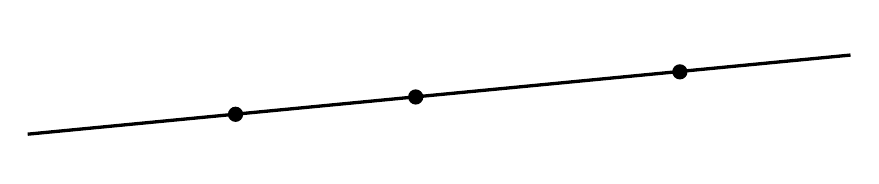
\begin{tikzpicture}[scale = 1.1]
    \clip(-3.6,1.24) rectangle (5.9,2.72);
    \draw [line width=1.2pt,domain=-3.6:5.9] plot(\x,{(--3.82--0.2*\x)/2.08});
    \begin{scriptsize}
        \fill (-1.2,1.72) circle (2.5pt);
        \fill (0.88,1.92) circle (2.5pt);
        \fill (3.93,2.21) circle (2.5pt);
    \end{scriptsize}
\end{tikzpicture}
        \end{figure}
        Al usar el teorema de \textbf{Menelao} tres veces en \theTriangle{XYZ}, primero con la transversal $A - B - M$, después con la transversal $P - C - D$ y finalmente con $F - N - E$, respectivamente, obtenemos que
        \begin{align*}
            &\ratioCM{X}{Y}{Z}{M}{A}{B} = 1,\\[3mm]
            &\ratioCM{X}{Y}{Z}{D}{P}{C} = 1\ \text{y}\\[3mm]
            &\ratioCM{X}{Y}{Z}{E}{F}{N} = 1.
        \end{align*}
    \end{multicols}
    \vspace{-10mm}
    Multiplicando estas tres igualdades y reordenando los miembros, obtenemos que
    \begin{align*}
        \ratioCM{X}{Y}{Z}{M}{P}{N} \cdot \frac{(YA\cdot YF) \cdot (ZB\cdot ZC) \cdot (XD\cdot XE)}{(AZ\cdot FZ) \cdot (BX \cdot CX) \cdot (DY\cdot EF)} = 1. \tag{$\ast$}
    \end{align*}
    Ahora por la \textbf{Propiedad~\ref{power-external-point}} sabemos que para los puntos $X$, $Y$ y $Z$ se cumple que
    \begin{align*}
        XD \cdot XE = XC \cdot XB \quad \land \quad
        YF \cdot YA = YE \cdot YD \quad \land \quad
        ZB \cdot ZC = ZA \cdot ZE
    \end{align*}
    Así $(\ast)$ se convierte en
    \[
        \ratioCM{X}{Y}{Z}{M}{P}{N} = 1,
    \]
    que por el teorema de \textbf{Menelao} significa que $M$, $N$ y $P$ son colineales.
\end{proof}

\begin{remark.tcb}
    Una manera fácil de recordar las intersecciones es la siguiente:
    Tomamos dos letras consecutivas, dejamos una letra de espacio, y tomamos otras dos letras consecutivas.
    La intersección de las rectas formadas con eso pares puntos es el primer punto de la colinealidad.
    Luego nos movemos a la derecha y repetimos el proceso dos veces más.\footnote{Otra manera de verlos es tomar vértices consecutivos módulo 3.}
    \begin{multicols}{2}
        \begin{figure}[H]
            \centering
            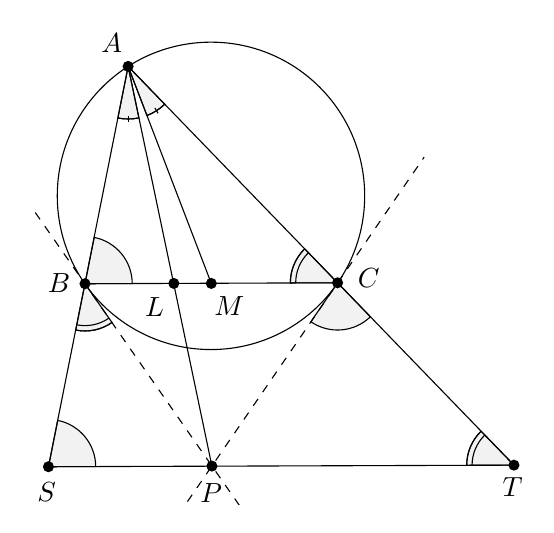
\begin{tikzpicture}[xscale = 0.4, yscale = 0.4]
    \clip(-2.36,-10.08) rectangle (13.47,5.06);
    \draw [shift={(-0.54,-3.07)},fill=black,fill opacity=0.05] (0,0) -- (0.2:1.5) arc (0.2:78.71:1.5) -- cycle;
    \draw [shift={(7.48,-3.04)},fill=black,fill opacity=0.05] (0,0) -- (-124.46:1.5) arc (-124.46:-45.95:1.5) -- cycle;
    \draw [shift={(-1.7,-8.88)},fill=black,fill opacity=0.05] (0,0) -- (0.2:1.5) arc (0.2:78.71:1.5) -- cycle;
    \draw [shift={(-0.54,-3.07)},fill=black,fill opacity=0.05] (0,0) -- (-101.29:1.5) arc (-101.29:-55.14:1.5) -- cycle;
    \draw [shift={(7.48,-3.04)},fill=black,fill opacity=0.05] (0,0) -- (134.05:1.5) arc (134.05:180.2:1.5) -- cycle;
    \draw [shift={(13.08,-8.83)},fill=black,fill opacity=0.05] (0,0) -- (134.05:1.5) arc (134.05:180.2:1.5) -- cycle;
    \draw [shift={(0.83,3.83)},fill=black,fill opacity=0.05] (0,0) -- (-101.29:1.67) arc (-101.29:-78.18:1.67) -- cycle;
    \draw [shift={(0.83,3.83)},fill=black,fill opacity=0.05] (0,0) -- (-69.06:1.67) arc (-69.06:-45.95:1.67) -- cycle;
    \draw(3.46,-0.28) circle (4.88cm);
    \draw (-0.54,-3.07)-- (7.48,-3.04);
    \draw (0.83,3.83)-- (-1.7,-8.88);
    \draw (0.83,3.83)-- (13.08,-8.83);
    \draw (-1.7,-8.88)-- (13.08,-8.83);
    \draw (0.83,3.83)-- (3.49,-8.86);
    \draw (0.83,3.83)-- (3.47,-3.06);
    \draw [dash pattern=on 3pt off 3pt,domain=-2.1176316762214267:13.472829432059696] plot(\x,{(-21.59-8.05*\x)/5.61});
    \draw [dash pattern=on 3pt off 3pt,domain=-2.361745286484902:10.226227746616733] plot(\x,{(--93.93-9.81*\x)/-6.74});
    \draw [shift={(-0.54,-3.07)}] (-101.29:1.5) arc (-101.29:-55.14:1.5);
    \draw [shift={(-0.54,-3.07)}] (-101.29:1.33) arc (-101.29:-55.14:1.33);
    \draw [shift={(7.48,-3.04)}] (134.05:1.5) arc (134.05:180.2:1.5);
    \draw [shift={(7.48,-3.04)}] (134.05:1.33) arc (134.05:180.2:1.33);
    \draw [shift={(13.08,-8.83)}] (134.05:1.5) arc (134.05:180.2:1.5);
    \draw [shift={(13.08,-8.83)}] (134.05:1.33) arc (134.05:180.2:1.33);
    \draw [shift={(0.83,3.83)}] (-101.29:1.67) arc (-101.29:-78.18:1.67);
    \draw(0.84,2.27) -- (0.84,2.07);
    \draw [shift={(0.83,3.83)}] (-69.06:1.67) arc (-69.06:-45.95:1.67);
    \draw(1.68,2.51) -- (1.78,2.34);
    \begin{scriptsize}
        \normalsize
        \fill [color=black] (0.83,3.83) circle (5pt);
        \draw[color=black] (0.31,4.56) node {$A$};
        \fill [color=black] (3.49,-8.86) circle (5pt);
        \draw[color=black] (3.47,-9.7) node {$P$};
        \fill [color=black] (-0.54,-3.07) circle (5pt);
        \draw[color=black] (-1.36,-3.04) node {$B$};
        \fill [color=black] (7.48,-3.04) circle (5pt);
        \draw[color=black] (8.47,-2.88) node {$C$};
        \fill [color=black] (-1.7,-8.88) circle (5pt);
        \draw[color=black] (-1.76,-9.68) node {$S$};
        \fill [color=black] (13.08,-8.83) circle (5pt);
        \draw[color=black] (13.04,-9.54) node {$T$};
        \fill [color=black] (2.28,-3.06) circle (5pt);
        \draw[color=black] (1.67,-3.81) node {$L$};
        \fill [color=black] (3.47,-3.06) circle (5pt);
        \draw[color=black] (4.04,-3.78) node {$M$};
    \end{scriptsize}
\end{tikzpicture}
            \caption{Teorema de Pascal.}
            \label{fig:pascal-theorem}
        \end{figure}
        \hfill\\
        \hfill\\
        \hfill\\
        \hfill
        \begin{figure}[H]
            \centering
            \begin{tabular}{|c|c|c|}
                \hline
                A & E & C\\\hline
                D & B & F\\
                \hline \hline
                N & P & M\\
                \hline
            \end{tabular}
            \caption{Mnemotécnia de Pascal.}
        \end{figure}

        Donde $N = \overline{EF} \cap \overline{CB}$, $P = \overline{AF} \cap \overline{CD}$ y $M = \overline{AB} \cap \overline{ED}$.
    \end{multicols}
\end{remark.tcb}


El~\refTheorem{\ref{t:pascal-theorem}} es independiente de cómo haya sido tomado el hexágono.
El mostrado en la demostración es el caso más sencillo en el cual el hexágono es convexo.
Sin embargo, la colinealidad se sigue cumpliendo aunque el hexágono no sea convexo, como se puede ver en la figura \ref{fig:pascal-theorem}.
La demostración de este caso y de cualquier otro es análoga a la primera.

\begin{section-example.tcb}{}{example-incenter}
    Sean $D$ y $E$ los puntos medios de los arcos menores $\wideparen{AB}$ y $\wideparen{AC}$ del circuncírculo del \theTriangle{ABC}, respectivamente.
    Sea $P$ un punto en el arco menor $BC$, $Q = PD \cap AB$ y $R = PE \cap AC$.
    Probar que la recta $QR$ pasa a traves de incentro $I$ del \theTriangle{ABC}.
\end{section-example.tcb}

\begin{solution}
    Dado que $D$ es el punto medio del arco $\wideparen{AB}$, $CD$ es bisectriz del ángulo $\angle BCA$.
    Análogamentes, $BE$ es bisectriz de $\angle ABC$.
    Por lo tanto, $CD \cap BE = I$.

    Ahora, aplicando el~\refTheorem{\ref{t:pascal-theorem}} al hexágono $CDPEBA$ tenemos que los puntos $CD \cap BE = I$, $DP \cap BA = Q$ y $PE \cap AC = R$ son colineales.
\end{solution}

\begin{figure}[H]
    \centering
    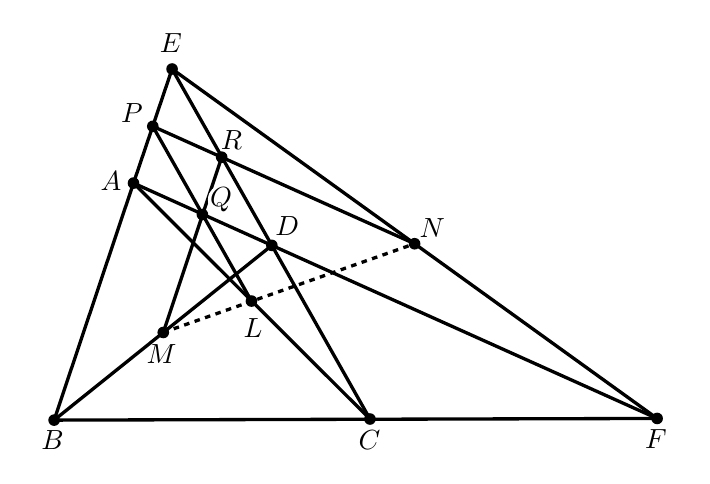
\begin{tikzpicture}[scale = 0.7]
    \clip(-1.74,-0.93) rectangle (10.12,6.84);
    \draw [line width=1.2pt] (-1.26,-0.28)-- (0.18,4.02);
    \draw [line width=1.2pt] (4.47,-0.26)-- (2.69,2.89);
    \draw [line width=1.2pt] (2.69,2.89)-- (0.18,4.02);
    \draw [line width=1.2pt] (-1.26,-0.28)-- (9.68,-0.25);
    \draw [line width=1.2pt] (2.69,2.89)-- (9.68,-0.25);
    \draw [line width=1.2pt] (2.69,2.89)-- (0.88,6.09);
    \draw [line width=1.2pt] (0.18,4.02)-- (0.88,6.09);
    \draw [line width=1.2pt] (0.88,6.09)-- (9.68,-0.25);
    \draw [line width=1.2pt] (-1.26,-0.28)-- (2.69,2.89);
    \draw [line width=1.2pt] (0.18,4.02)-- (4.47,-0.26);
    \draw [line width=1.2pt] (0.53,5.05)-- (2.32,1.88);
    \draw [line width=1.2pt] (1.78,4.49)-- (0.72,1.31);
    \draw [line width=1.2pt] (0.53,5.05)-- (5.28,2.92);
    \draw [line width=1.2pt,dash pattern=on 2pt off 2pt] (0.72,1.31)-- (5.28,2.92);
    \begin{scriptsize}
        \normalsize
        \fill [color=black] (0.18,4.02) circle (3.0pt);
        \draw[color=black] (-0.23,4.06) node {$A$};
        \fill [color=black] (-1.26,-0.28) circle (3.0pt);
        \draw[color=black] (-1.29,-0.65) node {$B$};
        \fill [color=black] (4.47,-0.26) circle (3.0pt);
        \draw[color=black] (4.46,-0.65) node {$C$};
        \fill [color=black] (2.69,2.89) circle (3.0pt);
        \draw[color=black] (2.97,3.24) node {$D$};
        \fill [color=black] (0.88,6.09) circle (3.0pt);
        \draw[color=black] (0.86,6.56) node {$E$};
        \fill [color=black] (9.68,-0.25) circle (3.0pt);
        \draw[color=black] (9.66,-0.63) node {$F$};
        \fill [color=black] (0.72,1.31) circle (3.0pt);
        \draw[color=black] (0.69,0.92) node {$M$};
        \fill [color=black] (2.32,1.88) circle (3.0pt);
        \draw[color=black] (2.35,1.39) node {$L$};
        \fill [color=black] (1.43,3.45) circle (3.0pt);
        \draw[color=black] (1.77,3.72) node[fill = white, rounded corners = 5pt, inner sep=0.8pt] {$Q$};
        \fill [color=black] (0.53,5.05) circle (3.0pt);
        \draw[color=black] (0.15,5.29) node {$P$};
        \fill [color=black] (1.78,4.49) circle (3.0pt);
        \draw[color=black] (1.96,4.81) node[fill = white, rounded corners = 5pt, inner sep=0.8pt] {$R$};
        \fill [color=black] (5.28,2.92) circle (3.0pt);
        \draw[color=black] (5.6,3.2) node {$N$};
    \end{scriptsize}
\end{tikzpicture}
    \caption{Ejemplo~\ref{e:example-incenter}, aplicación del teorema de Pascal.}
\end{figure}


El~\refTheorem{\ref{t:pascal-theorem}} puede presentar versiones degeneradas, aunque puede suceder, el caso más habitual ya no consiste en un paralelismo, sino en la transformación de un polígono de seis lados a un polígono de cinco, cuatro o tres lados.


%\begin{section-example.tcb}{}{}
%    Sea $\omega$ el circuncírculo del \theTriangle{ABC}.
%    Las tangentes a $\omega$ por lo puntos $A$, $B$ y $C$ intersecan a las rectas $BC$, $CA$ y $AB$ en los puntos $D$, $E$ y $F$, respectivamente.
%    Probar que los puntos $D$, $E$ y $F$ está alineados.
%\end{section-example.tcb}

%\begin{figure}[H]
%    \centering
%    \definecolor{qqqqcc}{rgb}{0,0,0.8}
%dash pattern=on 5pt off 2pt
%[fill = white, rounded corners = 5pt, inner sep=0.8pt]
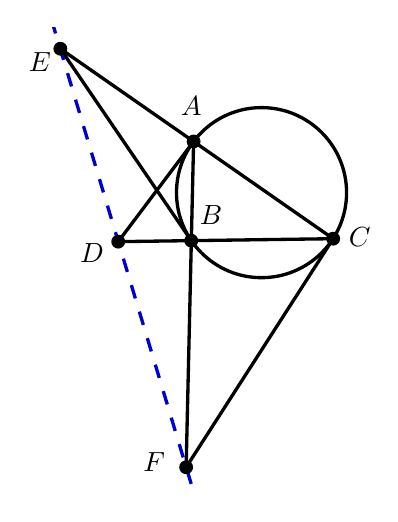
\begin{tikzpicture}[scale = 0.25]
    \clip(-10.02,-12.9) rectangle (7.34,10.77);
    \draw [line width=1.2pt] (1.86,2.39) circle (4.32cm);
    \draw [line width=1.2pt] (-8.36,9.7)-- (5.5,0.05);
    \draw [line width=1.2pt] (-8.36,9.7)-- (-1.71,-0.05);
    \draw [line width=1.2pt] (-5.42,-0.1)-- (5.5,0.05);
    \draw [line width=1.2pt] (-5.42,-0.1)-- (-1.59,4.99);
    \draw [line width=1.2pt] (-1.97,-11.56)-- (5.5,0.05);
    \draw [line width=1.2pt] (-1.97,-11.56)-- (-1.59,4.99);
    \draw [line width=1.2pt,dash pattern=on 5pt off 5pt,color=qqqqcc,domain=-10.02:7.34] plot(\x,{(-115.81-21.26*\x)/6.4});
    \begin{scriptsize}
        \normalsize
        \fill [color=black] (-1.59,4.99) circle (10.0pt);
        \draw[color=black] (-1.71,6.81) node {$A$};
        \fill [color=black] (-1.71,-0.05) circle (10pt);
        \draw[color=black] (-0.7,1.24) node {$B$};
        \fill [color=black] (5.5,0.05) circle (10pt);
        \draw[color=black] (6.85,0.11) node {$C$};
        \fill [color=black] (-8.36,9.7) circle (10pt);
        \draw[color=black] (-9.4,9) node {$E$};
        \fill [color=black] (-5.42,-0.1) circle (10pt);
        \draw[color=black] (-6.75,-0.69) node {$D$};
        \fill [color=black] (-1.97,-11.56) circle (10pt);
        \draw[color=black] (-3.59,-11.3) node {$F$};
    \end{scriptsize}
\end{tikzpicture}
%\end{figure}

%\begin{solution}
%    Aplicando el~\refTheorem{\ref{t:pascal-theorem}} al hexágono degenerado $AABBCC$.
%    Tenemos que los puntos $AA \cap BC = D$, $AB \cap CC = F$ y $BB \cap CA = E$ son colineales.
%\end{solution}

Existen $\dfrac{5!}{2} = 60$ maneras de posibles de formar un hexágono con 6 puntos distribuidos en una circunferencia, y, por el \refTheorem{\ref{t:pascal-theorem}}, a cada hexágono le corresponde una recta de Pascal.
Estas 60 rectas de Pascal pasan de tres en tres por 20 puntos llamados puntos de Steiner, que su vez están de cuatro en cuatro sobre 15 rectas, llamadas rectas de Plucker.



\subsection{Teorema de Brianchon}

\begin{section-theorem.tcb}{Teorema de Brianchon}{brianchon-theorem}
    Sea $ABCDEF$ un hexágono circunscrito, no necesariamente convexo, a un círculo $\Omega$.
    Entonces, las rectas $AD$, $BE$ y $CF$ son concurrentes.
\end{section-theorem.tcb}

\begin{figure}[H]
    \centering
    \definecolor{qqttzz}{rgb}{0,0.2,0.6}
\definecolor{ccqqqq}{rgb}{0.8,0,0}
\definecolor{qqqqcc}{rgb}{0,0,0.8}
\definecolor{qqqqzz}{rgb}{0,0,0.6}
\definecolor{wwwwww}{rgb}{0.4,0.4,0.4}

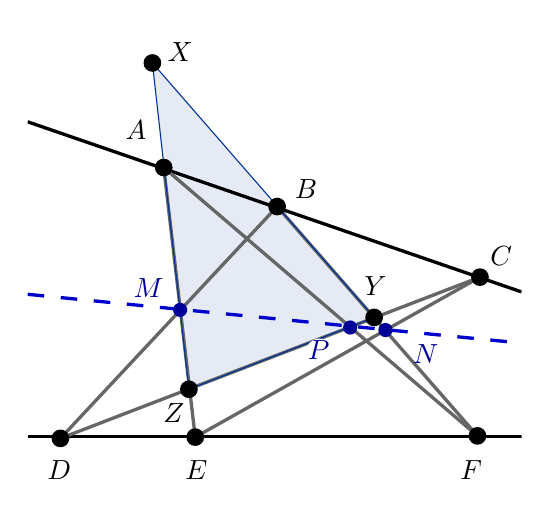
\begin{tikzpicture}[scale = 1.6]
    \clip(-2.86,1.38) rectangle (1.06,5.01);
    \fill[line width=0.4pt,color=qqttzz,fill=qqttzz,fill opacity=0.1] (-1.87,4.73) -- (-1.58,2.14) -- (-0.11,2.71) -- cycle;
    \draw [line width=1.2pt,domain=-2.86:1.06] plot(\x,{(--2.95-0.31*\x)/0.9});
    \draw [line width=1.2pt,domain=-2.86:1.06] plot(\x,{(--1.87-0*\x)/1.06});
    \draw [line width=1.2pt,color=wwwwww] (-1.78,3.9)-- (-1.53,1.76);
    \draw [line width=1.2pt,color=wwwwww] (-1.78,3.9)-- (0.71,1.77);
    \draw [line width=1.2pt,color=wwwwww] (-2.6,1.75)-- (-0.88,3.59);
    \draw [line width=1.2pt,color=wwwwww] (-2.6,1.75)-- (0.73,3.03);
    \draw [line width=1.2pt,color=wwwwww] (-1.53,1.76)-- (0.73,3.03);
    \draw [line width=1.2pt,color=wwwwww] (-0.88,3.59)-- (0.71,1.77);
    \draw [line width=1.2pt,dash pattern=on 6pt off 6pt,color=qqqqcc,domain=-2.86:1.06] plot(\x,{(--4.23-0.16*\x)/1.62});
    \draw [line width=0.4pt,color=qqttzz] (-1.87,4.73)-- (-1.58,2.14);
    \draw [line width=0.4pt,color=qqttzz] (-1.58,2.14)-- (-0.11,2.71);
    \draw [line width=0.4pt,color=qqttzz] (-0.11,2.71)-- (-1.87,4.73);
    \begin{scriptsize}
        \normalsize
        \fill [color=black] (-1.78,3.9) circle (2.0pt);
        \draw[color=black] (-2, 4.2) node {$A$};
        \fill [color=black] (-0.88,3.59) circle (2.0pt);
        \draw[color=black] (-0.65,3.73) node {$B$};
        \fill [color=black] (0.73,3.03) circle (2.0pt);
        \draw[color=black] (0.9,3.2) node {$C$};
        \fill [color=black] (-2.6,1.75) circle (2.0pt);
        \draw[color=black] (-2.61,1.5) node {$D$};
        \fill [color=black] (-1.53,1.76) circle (2.0pt);
        \draw[color=black] (-1.52,1.5) node {$E$};
        \fill [color=black] (0.71,1.77) circle (2.0pt);
        \draw[color=black] (0.66,1.5) node {$F$};
        \fill [color=qqqqzz] (-1.65,2.77) circle (1.6pt);
        \draw[color=qqqqzz] (-1.9,2.94) node {$M$};
        \fill [color=qqqqzz] (-0.3,2.63) circle (1.6pt);
        \draw[color=qqqqzz] (-0.55,2.45) node[fill = white, rounded corners = 5pt, inner sep=0.8pt] {$P$};
        \fill [color=qqqqzz] (-0.02,2.61) circle (1.6pt);
        \draw[color=qqqqzz] (0.30,2.42) node {$N$};
        \fill [color=black] (-1.87,4.73) circle (2.0pt);
        \draw[color=black] (-1.65,4.82) node {$X$};
        \fill [color=black] (-1.58,2.14) circle (2.0pt);
        \draw[color=black] (-1.70,1.95) node {$Z$};
        \fill [color=black] (-0.11,2.71) circle (2.0pt);
        \draw[color=black] (-0.10,2.96) node {$Y$};
    \end{scriptsize}
\end{tikzpicture}
    \caption{Teorema de Brianchon.}
\end{figure}

La demostración más sencilla del teorema de Brianchon implica utilizar polos y polares.
Pues resulta que el~\refTheorem{\ref{t:pascal-theorem}} y \refTheorem{\ref{t:brianchon-theorem}} son \textit{duales bajo la transformación polar}.
Esto significa que, al tomar la colinealidad proporcionada por el~\refTheorem{\ref{t:pascal-theorem}} y aplicarle la transformación polar con respecto al círculo de referencia, inmediatamente obtenemos la concurrencia que el~\refTheorem{\ref{t:brianchon-theorem}} implica.
Ya que el tema de polos y polares no lo veremos en el curso, se invita al estudiante indagar la demostración de este teorema por su cuenta.

De la misma manera que con el primer teorema, el~\refTheorem{\ref{t:brianchon-theorem}} está sujeto a versiones degeneradas.
En este caso, los vértices degenerados coinciden con los puntos de tangencia entre el polígono y el círculo inscrito.
En efecto, al aplicar el~\refTheorem{\ref{t:brianchon-theorem}} al hexagono $ABCDEF$ con $D$, $F$ y $B$ puntos de tangencia, como se muestra en la figura~\ref{fig:case-briancho-theorem}, redescubrimos que los puntos de tangencia del incírculo de \theTriangle{ACE} concurren.

\begin{figure}[H]
    \centering
    \definecolor{ttttff}{rgb}{0.2,0.2,1}
%dash pattern=on 5pt off 2pt
%[fill = white, rounded corners = 5pt, inner sep=0.8pt]
\begin{tikzpicture}[scale = 0.65]
    \clip(8.45,-6.14) rectangle (23.62,4.58);
    \draw [line width=1.2pt] (15.6,-3.7) circle (1.05cm);
    \draw [line width=1.2pt] (10.53,0.69) circle (1.9cm);
    \draw [line width=1.2pt] (19.73,0.87) circle (3.51cm);
    \draw [dash pattern=on 6pt off 6pt,domain=8.45:23.62] plot(\x,{(--25.45-1.98*\x)/0.84});
    \draw [dash pattern=on 6pt off 6pt,domain=8.45:23.62] plot(\x,{(--3.14-0.55*\x)/2.08});
    \draw [dash pattern=on 6pt off 6pt,domain=8.45:23.62] plot(\x,{(-22.13--1.49*\x)/-2.14});
    \draw [dash pattern=on 6pt off 6pt,domain=8.45:23.62] plot(\x,{(--20.12-1.58*\x)/-2.08});
    \draw [dash pattern=on 6pt off 6pt,domain=8.45:23.62] plot(\x,{(-26.17--0.99*\x)/2.19});
    \draw [dash pattern=on 6pt off 6pt,domain=8.45:23.62] plot(\x,{(-35.94--2.28*\x)/0.77});
    \draw [line width=0.8pt, dash pattern=on 6pt off 2pt,color=ttttff,domain=8.45:23.62] plot(\x,{(-88.14--6.4*\x)/-0.09});
    \begin{scriptsize}
        \normalsize
        \fill [color=black] (15.6,-3.7) circle (4pt);
        \draw[color=black] (15.98,-3.18) node {$O_1$};
        \fill [color=black] (19.73,0.87) circle (4pt);
        \draw[color=black] (20.25,1.41) node {$O_2$};
        \fill [color=black] (10.53,0.69) circle (4pt);
        \draw[color=black] (11.01,1.18) node {$O_3$};
        \fill [color=black] (13.84,-5.65) circle (4pt);
        \draw[color=black] (13.28,-5.1) node {$P_1$};
        \fill [color=black] (13.79,-2.14) circle (4pt);
        \draw[color=black] (13.1,-1.41) node {$Q_2$};
        \fill [color=black] (13.76,0.75) circle (4pt);
        \draw[color=black] (13.19,1.76) node {$Q_3$};
    \end{scriptsize}
\end{tikzpicture}
    \caption{Un caso degenerado del teorema de Brianchon.}
    \label{fig:case-briancho-theorem}
\end{figure}

\begin{remark.tcb}
    Al igual que con el teorema anterior, existe una manera fácil de obtener el punto de concurrencia.
    Ordenamos los puntos en una tabla, luego tomamos los segmentos formados con los puntos consecutivos de arriba hacia abajo.
    La intersección de estos segmentos es el punto de concurrencia.
    \begin{figure}[H]
        \centering
        \begin{tabular}{|c|c|c|}
            \hline
            A & B & C\\\hline
            D & E & F\\
            \hline \hline
            AD & BE & CF \\
            \hline
        \end{tabular}
        \caption{Mnemotécnia de Brianchon.}
    \end{figure}
    Es decir $P = \overline{AD} \cap \overline{BE} \cap \overline{CF}$.
    Otra manera de ver esto, es tomar las rectas formadas por los puntos cuyas posiciones son las mismas en módulo 3.
\end{remark.tcb}



\section{Conocimiento previo}

\begin{section-property}[Potencia de un punto exterior]\label{power-external-point}
Sean $AD$ y $CD$ dos rectas que se intersecan en $X$ tales que $X - A - B$ y $X - C - D$.
Entonces el cuadrilátero $ABCD$ es cíclico si y solo si
\[
    \overline{XA} \cdot \overline{XB} = \overline{XC} \cdot \overline{XD}.
\]
\end{section-property}

\begin{multicols}{2}
    \begin{proof}
        Rápidamente nos damos cuenta de que $\angle CXB = \angle AXD\quad (\ast).$

        Entonces $ABCD$ es cíclico
        \begin{align*}
            &\iff \angle ABC = \angle ADC\\
            &\iff \angle XBC = \angle ADX\\
            &\overset{(\ast)}{\iff} \triangle XBC \sim \triangle XDA \ \overset{(\ast)}{\iff} \ \frac{\overline{XB}}{\overline{XC}} = \frac{\overline{XD}}{\overline{XA}}\\[2mm]
            &\iff \overline{XA} \cdot \overline{XB} = \overline{XC} \cdot \overline{XD}. \qedhere
        \end{align*}
    \end{proof}
    \begin{figure}[H]
        \centering
        \definecolor{ttttff}{rgb}{0.2,0.2,1}
%dash pattern=on 5pt off 2pt
%[fill = white, rounded corners = 4pt, inner sep = 1pt]
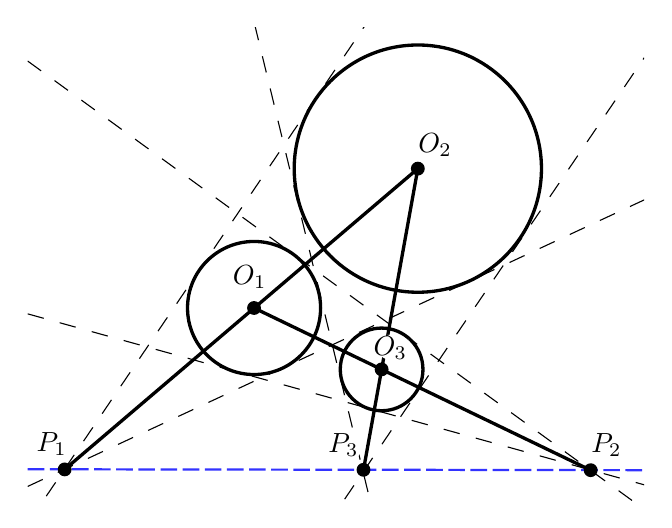
\begin{tikzpicture}[scale = 0.5]
    \clip(4.47,-5.82) rectangle (20.13,6.18);
    \draw [line width=1.2pt] (10.22,-0.94) circle (1.69cm);
    \draw [line width=1.2pt] (13.46,-2.5) circle (1.05cm);
    \draw [line width=1.2pt] (14.38,2.6) circle (3.14cm);
    \draw [line width=1.2pt] (5.41,-5.04)-- (14.38,2.6);
    \draw [line width=1.2pt] (14.38,2.6)-- (13,-5.05);
    \draw [line width=1.2pt] (10.22,-0.94)-- (18.77,-5.06);
    \draw [color = ttttff, dash pattern=on 6pt off 2pt, line width=0.8pt, domain=4.47:20.13] plot(\x,{(-67.19-0.02*\x)/13.36});
    \draw [dash pattern=on 6pt off 6pt,domain=4.47:20.13] plot(\x,{(-41.75--2.57*\x)/5.53});
    \draw [dash pattern=on 6pt off 6pt,domain=4.47:20.13] plot(\x,{(-44.52--5.05*\x)/3.42});
    \draw [dash pattern=on 6pt off 6pt,domain=4.47:20.13] plot(\x,{(-32.25--1.96*\x)/1.33});
    \draw [dash pattern=on 6pt off 6pt,domain=4.47:20.13] plot(\x,{(-27.15--2.31*\x)/-0.56});
    \draw [dash pattern=on 6pt off 6pt,domain=4.47:20.13] plot(\x,{(-40.25--3.41*\x)/-4.69});
    \draw [dash pattern=on 6pt off 6pt,domain=4.47:20.13] plot(\x,{(-0.84--1.55*\x)/-5.59});
    \begin{scriptsize}
        \normalsize
        \fill [color=black] (10.22,-0.94) circle (5pt);
        \draw[color=black] (10.11,-0.15) node[fill = white, rounded corners = 4pt, inner sep = 1pt] {$O_1$};
        \fill [color=black] (14.38,2.6) circle (5pt);
        \draw[color=black] (14.82,3.2) node {$O_2$};
        \fill [color=black] (13.46,-2.5) circle (5pt);
        \draw[color=black] (13.68,-1.95) node[fill = white, rounded corners = 8pt, inner sep = 0.5pt] {$O_3$};
        \fill [color=black] (5.41,-5.04) circle (5pt);
        \draw[color=black] (5.08,-4.4) node {$P_1$};
        \fill [color=black] (18.77,-5.06) circle (5pt);
        \draw[color=black] (19.17,-4.43) node {$P_2$};
        \fill [color=black] (13,-5.05) circle (5pt);
        \draw[color=black] (12.49,-4.43) node[fill = white, rounded corners = 4pt, inner sep = 1pt] {$P_3$};
    \end{scriptsize}
\end{tikzpicture}
    \end{figure}
\end{multicols}




\section{Ejercicios y Problemas}

Sección de ejercicios y problemas para el autoestudio.

\begin{section-problem}
    Dado el \theTriangle{ABC} con circuncentro $O$.
    Sea $A_1$ y $B_1$ los pies de las alturas trazadas desde $A$ y $B$, respectivamente.
    Sea $M$ y $N$ los puntos medios de $AC$ y $BC$, respectivamente.
    Sea el punto $X \in BB_1$ tal que $MX \perp AB$ y de manera análoga el punto $Y \in AA_1$ tal que $NY \perp AB$.
    Se define $P = A_1 M \cap B_1 N$ y $Q = XN \cap YM$.
    Demostrar que $P$, $Q$ y $O$ son colineales.
\end{section-problem}

\begin{section-problem}
    Sea \theTriangle{ABC} un triángulo acutángulo y $\Gamma$ su circuncírculo.
    Sea $D$ un punto en el segmento $BC$, diferente de $B$ y $C$, y sea $M$ el punto medio de $AD$.
    La perpendicular a $AB$ que pasa por $D$ interseca a $AB$ en $E$ y $\Gamma$ en $F$, con el punto $D$ entre $E$ y $F$.
    Las rectas $FC$ y $EM$ se intersectan en el punto $X$.
    Si $\angle DAE = \angle AFE$, demostrar que la recta $AX$ es tangente a $\Gamma$.
\end{section-problem}

\begin{section-problem}
    Sea $\Gamma$ el circuncírculo del \theTriangle{ABC}.
    Un círculo que pasa por $A$ y $C$ corta a los lados $BC$ y $BA$ en $D$ y $E$, respectivamente.
    Las rectas $AD$ y $CE$ intersecan a $\Gamma$ por segunda vez en $G$ y $H$, respectivamente.
    Las tangentes a $\Gamma$ por $A$ y $C$ intersecan a la recta $DE$ en $L$ y $M$, respectivamente.
    Probar que las rectas $LH$ y $MG$ se cortan en $\Gamma$.
\end{section-problem}

\begin{section-problem}
    Sea el triángulo \theTriangle{ABC} y sean $D$, $E$ y $F$ los puntos de tangencia del excírculo en $A$ con respecto a los lados $BC$, $CA$ y $AB$.
    Sean $H$ y $G$ las intersecciones de excírculo con $BE$ y $CF$ respectivamente.
    Se toma un punto $S$ en $AD$, sean $U$ y $V$ las intersecciones del excírculo con $SH$ y $SG$ respectivamente.
    Demuestre que $BC$, $UV$, $GH$ y $EF$ son concurrentes.
\end{section-problem}